\section{HP Causality}

\subsection{Minimal Enabling as a Cause}

\begin{thm}\label{thm:hp-x-y}
Given an event structure $\es$, a cause $X = S \vdash\,e$
where $(S, e) \in \vdash$, and an effect $Y = S_f$
where $S_f \in \conf{\es}$, $X$ is a cause of $Y$
(according to the HP definition) if there is at least one path
from $m_{S,e}$ to $x_{S_f}$ in the causal graph of $\es$.
\end{thm}

\begin{proof}
We check the conditions of HP causality for the given cause and effect.

\begin{itemize}
  \item \textbf{AC1:} Both the cause and effect hold in the factual scenario;
  therefore, this condition is satisfied.
\end{itemize}

For AC2.\{a,b\}, assume $(W, w, x')$ is the witness discussed by HP.

\begin{itemize}  
  \item \textbf{AC2.a:} The idea here is to restrict the causal graph
  such that the effect holds as long as the cause.
  
  Assume the path from cause to effect is as follows:
  \begin{equation}\label{eq:validating-path}
    m_{S,e} \rightarrow
    r_{S_1,S_2} \rightarrow
    x_{S_2} \rightarrow
    r_{S_2, S_3} \rightarrow
    \cdots \rightarrow
    r_{S_{k-1}, S_k} \rightarrow x_{S_k} = x_{S_f}
  \end{equation}

  We also define $W$ as:
  \[ \left( \In{r_{S_1, S_2}} \setminus \set{x_{S_1}, m_{S,e}} \right) \cup
    \left( \bigcup_{i=2}^k \In{x_{S_i}} \setminus \set{r_{S_{i-1}, S_i}} \right) \]
   
  The elements of $W$ are shown with dotted boxes in Fig. \ref{fig:witness}.
  All variables in $W$ are set to False ($w$ is an all-False valuation).
  $x'$ sets $r_{S,e}$ to False as well.
  
  \textbf{The choice of $W$ and validating path:}
  By defining $W$ as explained above, and setting it to all-False,
  the value for each vertex of the \textit{validating} path
  (as shown in Eq. \ref{eq:validating-path})
  can be determined by its predecessor. For $i \geq 2$, we have:
  \begin{equation}\label{eq:x-Si-restrict}
    x_{S_i} = r_{S_{i-1}, S_i}
  \end{equation}
  
  By definition, each reason vertex consists of
  an \textit{enabling} and a \textit{configuration} component.
  We know the validating path is in the causal graph. Hence, for $i \geq 2$,
  the enabling component for $r_{S_i, S_{i+1}}$ is satisfied; so we have:
  \begin{equation}\label{eq:r-Si-Si+1-restrict}
    r_{S_i, S_{i+1}} = x_{S_i} \wedge \text{True} = x_{S_i}
  \end{equation}
  
  For $r_{S_1,S_2}$, after setting $W$ to all-False, we have:
  \begin{equation}\label{eq:r-S1-S2-restrict}
    r_{S_1,S_2} = \text{True} \wedge m_{S,e} = m_{S,e}
  \end{equation}
  
  \begin{figure}
\centering
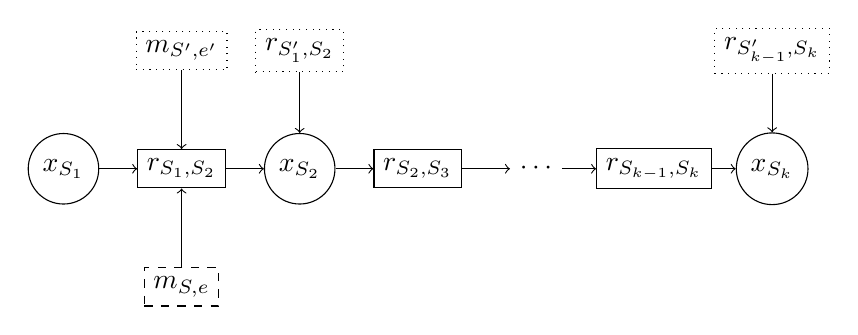
\begin{tikzpicture}
  \tikzset{
    _x/.style={circle,draw},
    r/.style={rectangle,draw},
    m/.style={rectangle,draw,dashed},
    w/.style={rectangle,draw,dotted},
  };
  \node[_x] (x-S1)       at (-1.5,0)  {$x_{S_1}$};
  \node[_x] (x-S2)       at (1.5,0)   {$x_{S_2}$};
  \node[_x] (x-Sk)       at (7.5,0)   {$x_{S_k}$};
  \node[m]  (m-S-e)      at (0,-1.5)  {$m_{S,e}$};
  \node[r]  (r-S1-S2)    at (0,0)     {$r_{S_1,S_2}$};
  \node[r]  (r-S2-S3)    at (3,0)     {$r_{S_2,S_3}$}; 
  \node[r]  (r-Sk-1-Sk)  at (6,0)     {$r_{S_{k-1},S_k}$};
  \node[w]  (m-S'-e')    at (0,1.5)   {$m_{S',e'}$};
  \node[w]  (r-S'1-S2)   at (1.5,1.5) {$r_{S'_1,S_2}$};
  \node[w]  (r-S'k-1-Sk) at (7.5,1.5) {$r_{S'_{k-1},S_k}$};
  \node     (dots)       at (4.5,0)   {$\cdots$};

  \draw[->] (x-S1)       -- (r-S1-S2);
  \draw[->] (m-S-e)      -- (r-S1-S2);
  \draw[->] (m-S'-e')    -- (r-S1-S2);
  \draw[->] (r-S1-S2)    -- (x-S2);
  \draw[->] (r-S'1-S2)   -- (x-S2);
  \draw[->] (x-S2)       -- (r-S2-S3);
  \draw[->] (r-S2-S3)    -- (dots);
  \draw[->] (dots)       -- (r-Sk-1-Sk);
  \draw[->] (r-Sk-1-Sk)  -- (x-Sk);
  \draw[->] (r-S'k-1-Sk) -- (x-Sk);
\end{tikzpicture}
\caption{Elements of $W$}
\label{fig:witness}
\end{figure}
    

  As shown in Eqs.
  \ref{eq:x-Si-restrict}, \ref{eq:r-Si-Si+1-restrict}, \ref{eq:r-S1-S2-restrict},
  Setting $m_{S,e}$ to False and $W$ to all-False will set all vertices
  in the validating path to False.

  With the witness described above, we can see that the effect $x_{S_f}$
  is also valuated as False; therefore, condition AC2.a is satisfied.
  
  
  \item \textbf{AC2.b:} After setting $m_{S,e}$ to True,
  while maintaining $W$ as all-False, $x_{S_f}$ is valuated to True again;
  this follows from the equations of the validating path when $W$ is set to all-False.
  The \textit{validating edges} for $x_{S_f}$ are shown with thick lines
  in Fig. \ref{fig:ac2.b}. Observe that, re-setting any variable $v \not\in W$
  does \textbf{not} \textit{invalidate} the specified path for $x_{S_f}$.

  \begin{figure}
\centering
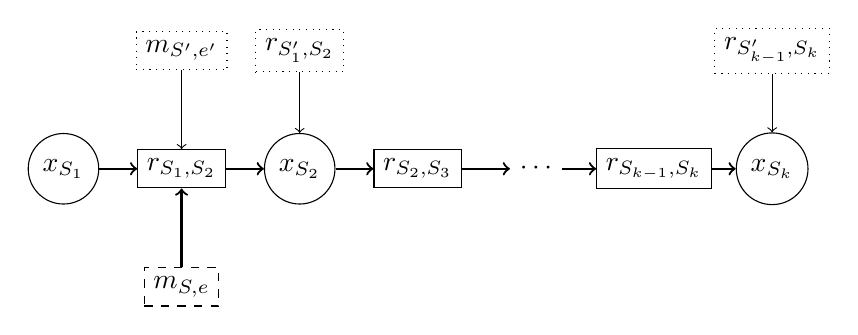
\begin{tikzpicture}
  \tikzset{
    _x/.style={circle,draw},
    r/.style={rectangle,draw},
    m/.style={rectangle,draw,dashed},
    w/.style={rectangle,draw,dotted},
  };
  \node[_x] (x-S1)       at (-1.5,0)  {$x_{S_1}$};
  \node[_x] (x-S2)       at (1.5,0)   {$x_{S_2}$};
  \node[_x] (x-Sk)       at (7.5,0)   {$x_{S_k}$};
  \node[m]  (m-S-e)      at (0,-1.5)  {$m_{S,e}$};
  \node[r]  (r-S1-S2)    at (0,0)     {$r_{S_1,S_2}$};
  \node[r]  (r-S2-S3)    at (3,0)     {$r_{S_2,S_3}$}; 
  \node[r]  (r-Sk-1-Sk)  at (6,0)     {$r_{S_{k-1},S_k}$};
  \node[w]  (m-S'-e')    at (0,1.5)   {$m_{S',e'}$};
  \node[w]  (r-S'1-S2)   at (1.5,1.5) {$r_{S'_1,S_2}$};
  \node[w]  (r-S'k-1-Sk) at (7.5,1.5) {$r_{S'_{k-1},S_k}$};
  \node     (dots)       at (4.5,0)   {$\cdots$};

  \draw[->,thick] (x-S1)       -- (r-S1-S2);
  \draw[->,thick] (m-S-e)      -- (r-S1-S2);
  \draw[->] (m-S'-e')    -- (r-S1-S2);
  \draw[->,thick] (r-S1-S2)    -- (x-S2);
  \draw[->] (r-S'1-S2)   -- (x-S2);
  \draw[->,thick] (x-S2)       -- (r-S2-S3);
  \draw[->,thick] (r-S2-S3)    -- (dots);
  \draw[->,thick] (dots)       -- (r-Sk-1-Sk);
  \draw[->,thick] (r-Sk-1-Sk)  -- (x-Sk);
  \draw[->] (r-S'k-1-Sk) -- (x-Sk);
\end{tikzpicture}
\caption{\textit{Validating} path for $X_{S_f}$}
\label{fig:ac2.b}
\end{figure}
    

  \item \textbf{AC3:} As our cause is a singleton,
  this condition is also satisfied.
\end{itemize}

\end{proof}

\begin{thm}\label{thm:hp-x-disj-Y}
Given an event structure $\es$, a cause $X = S \vdash\,e$
where $(S, e) \in \vdash$, and an effect $Y = \bigvee_{f} S_{f}$
where $\forall f.\;S_f \in \conf{\es}$, $X$ is a cause of $Y$
(according to the HP definition) if there exists $f$ such that
there is at least one path from $m_{S,e}$ to $x_{S_f}$
in the causal graph of $\es$.
\end{thm}

\begin{proof}
Assume there is a path from $m_{S,e}$ to $x_{S_f}$ for some $f$.
Also assume $W$ is defined as in Thm. \ref{thm:hp-x-y}. For this problem,
we construct the new witness $W'$ as follows:
\[ W' = W \cup \left( \bigcup_{f' \neq f} x_{S_{f'}} \right) \]

$W'$ is set to all-False, as before.

With the new witness, both AC2.a and AC2.b can be satisfied
for the new problem.
\end{proof}

\begin{thm}\label{thm:hp-x-conj-Y}
Given an event structure $\es$, a cause $X = S \vdash\,e$
where $(S, e) \in \vdash$, and an effect $Y = \bigwedge_{f} S_{f}$
where $\forall f.\;S_f \in \conf{\es}$, $X$ is a cause of $Y$
(according to the HP definition) if there exists $f$ such that
there is at least one path from $m_{S,e}$ to $x_{S_f}$
in the causal graph of $\es$.  
\end{thm}

\begin{proof}
The set $W$ is selected just as done in Thm. \ref{thm:hp-x-disj-Y}.
For any $w \in W \cap Y$, we set $w$ to True.
\end{proof}

\begin{thm}\label{thm:hp-X-Y}
Given an event structure $\es$,
a cause $X = \set{S_1 \vdash\, e_1, \cdots, S_k \vdash\, e_k}$
where $(S_i, e_i) \in \vdash$, and an effect $Y = x_{S_f}$
where $S_f \in \conf{\es}$, $X$ is not a cause of $Y$. 
\end{thm}

\begin{proof}
The result holds if there is no path from $X$ to $Y$.
Assume there is a path from $X$ to $Y$.
this path starts from a vertex $m_{S_i,e_i}$, where $(S_i \vdash e_i) \in X$.
As stated in Thm. \ref{thm:hp-x-y}, $S_i \vdash e_i$ is a cause of $Y$.
Hence, AC3 does not hold for $X$.
\end{proof}

\subsection{False Minimal Enabling as a Cause}

In the previous section, we showed how to check causality for
true minimal enabling relations
(i.e. $S \vdash e =$ True in the given event structure).
Now we want to improve the existing causal graph
to include false minimal enabling relations as well.

Given event structure $\es = (E, \#, \vdash)$,
For each $S \subseteq E$ and $e \in E$, we define vertex $r_{S,e}$.
The value associated with this vertex will be as follows:

\[ m_{S,e} =
  \begin{cases}
    \Min{S}{e}   & \text{if } S \vdash_{min} e \\
    \text{False} & \text{otherwise}
  \end{cases}
\]

Where $\Min{S}{e}$ is defined as follows:
\[ \Min{S}{e} =
  \bigwedge_{S' \subseteq E.\;(S' \subset S) \vee (S \subset S')}
  \neg m_{S',e}
\]

Informally, if $S$ minimally enables $e$, no pure sub- or super-set of $S$
minimally enables $e$. 